\documentclass[12pt]{article}
\usepackage{amsmath, amssymb}
\usepackage{graphicx}
\usepackage{listings}
\usepackage{xcolor}
\usepackage{hyperref}
\usepackage{geometry}
\geometry{a4paper, margin=1in}

\definecolor{codegray}{rgb}{0.95,0.95,0.95}
\lstset{
  backgroundcolor=\color{codegray},
  basicstyle=\ttfamily\footnotesize,
  frame=single,
  breaklines=true,
  postbreak=\mbox{\textcolor{red}{$\hookrightarrow$}\space},
  keywordstyle=\color{blue},
  commentstyle=\color{gray},
  stringstyle=\color{red},
}

\title{\textbf{Experiment 5: Analysis of Distribution Function Z = X\textsubscript{1} + X\textsubscript{2}}}
\author{Your Name}
\date{28 July 2025}

\begin{document}

\maketitle

\section*{Objective}
To study the distribution of a random variable \( Z = X_1 + X_2 \), where \( X_1 \) and \( X_2 \) are independently drawn from:
\begin{itemize}
  \item Uniform distributions
  \item Normal distributions
\end{itemize}
and to observe the effect of different combinations of ranges and parameters on the distribution of \( Z \) using simulations in Python.

\section*{Problem Statement}
Consider a distribution function \( Z \) where:
\[
Z = X_1 + X_2
\]
with \( X_1 \) and \( X_2 \) being random variables generated using the \texttt{rvs} function from the \texttt{scipy.stats} library.

\subsection*{Tasks}
\begin{enumerate}
  \item[A)] Uniform Distribution
    \begin{enumerate}
      \item[i)] \( X_1, X_2 \sim U(0, 1) \)
      \item[ii)] \( X_1 \sim U(0, 1), X_2 \sim U(0, 2) \)
    \end{enumerate}
  \item[B)] Normal Distribution
    \begin{enumerate}
      \item[i)] \( X_1, X_2 \sim N(0, 1) \)
      \item[ii)] \( X_1 \sim N(0, 1), X_2 \sim N(0, 4) \)
    \end{enumerate}
\end{enumerate}

\section*{Theory}
\subsection*{Sum of Independent Random Variables}
If \( X_1 \) and \( X_2 \) are independent random variables:
\begin{itemize}
  \item For uniform distributions, the sum \( Z \) follows a triangular-like distribution.
  \item For normal distributions, the sum \( Z \) also follows a normal distribution with:
  \[
  \mu_Z = \mu_1 + \mu_2, \quad \sigma_Z = \sqrt{\sigma_1^2 + \sigma_2^2}
  \]
\end{itemize}

\section*{Python Code and Results}

\subsection*{A) Uniform Distributions}

\subsubsection*{Case i: \( X_1, X_2 \sim U(0,1) \)}
\begin{lstlisting}[language=Python]
from scipy.stats import uniform
import matplotlib.pyplot as plt
import numpy as np

n = 100000
X1 = uniform.rvs(loc=0, scale=1, size=n)
X2 = uniform.rvs(loc=0, scale=1, size=n)
Z = X1 + X2

plt.hist(Z, bins=100, density=True, alpha=0.7, color='skyblue', edgecolor='black')
plt.title('Z = X1 + X2, X1,X2 ~ U(0,1)')
plt.xlabel('Z')
plt.ylabel('Density')
plt.grid(True)
plt.show()
\end{lstlisting}

\textbf{Output:} \\
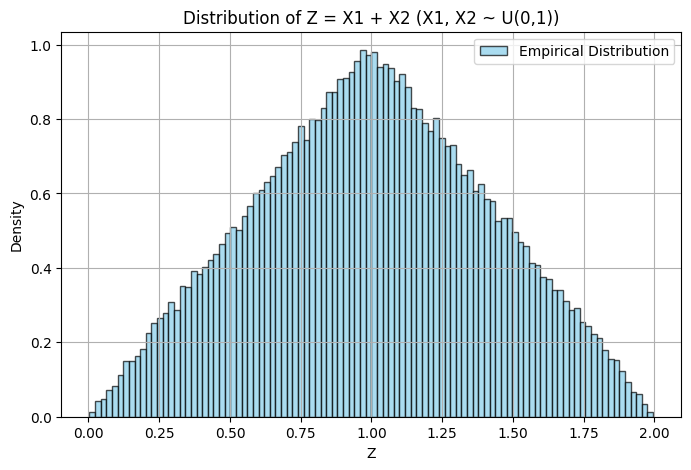
\includegraphics[width=0.8\linewidth]{uniform_0_1.png}

\subsubsection*{Case ii: \( X_1 \sim U(0,1), X_2 \sim U(0,2) \)}
\begin{lstlisting}[language=Python]
X1 = uniform.rvs(loc=0, scale=1, size=n)
X2 = uniform.rvs(loc=0, scale=2, size=n)
Z = X1 + X2

plt.hist(Z, bins=100, density=True, alpha=0.7, color='salmon', edgecolor='black')
plt.title('Z = X1 + X2, X1 ~ U(0,1), X2 ~ U(0,2)')
plt.xlabel('Z')
plt.ylabel('Density')
plt.grid(True)
plt.show()
\end{lstlisting}

\textbf{Output:} \\
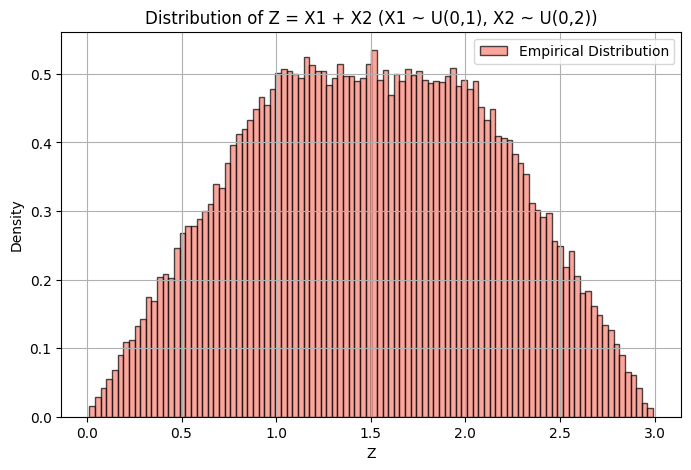
\includegraphics[width=0.8\linewidth]{uniform_0_2.png}

\newpage
\subsection*{B) Normal Distributions}

\subsubsection*{Case i: \( X_1, X_2 \sim N(0,1) \)}
\begin{lstlisting}[language=Python]
from scipy.stats import norm

mu1, sigma1 = 0, 1
mu2, sigma2 = 0, 1

X1 = norm.rvs(loc=mu1, scale=sigma1, size=n)
X2 = norm.rvs(loc=mu2, scale=sigma2, size=n)
Z = X1 + X2

mu_z = mu1 + mu2
sigma_z = np.sqrt(sigma1**2 + sigma2**2)

plt.hist(Z, bins=100, density=True, alpha=0.6, color='lightgreen', edgecolor='black')
x = np.linspace(min(Z), max(Z), 1000)
pdf = norm.pdf(x, loc=mu_z, scale=sigma_z)
plt.plot(x, pdf, 'r--', label=f'N({mu_z}, {sigma_z:.2f}²)')
plt.title('Z = X1 + X2, X1,X2 ~ N(0,1)')
plt.xlabel('Z')
plt.ylabel('Density')
plt.legend()
plt.grid(True)
plt.show()
\end{lstlisting}

\textbf{Output:} \\
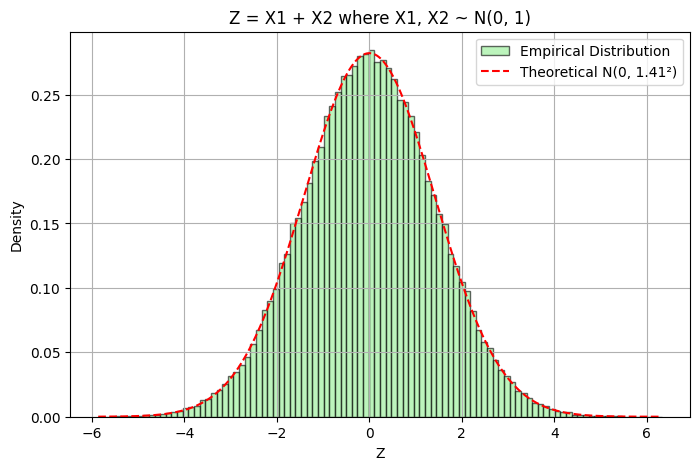
\includegraphics[width=0.8\linewidth]{normal_0_1.png}

\subsubsection*{Case ii: \( X_1 \sim N(0,1), X_2 \sim N(0,4) \)}
\begin{lstlisting}[language=Python]
mu1, sigma1 = 0, 1
mu2, sigma2 = 0, 2

X1 = norm.rvs(loc=mu1, scale=sigma1, size=n)
X2 = norm.rvs(loc=mu2, scale=sigma2, size=n)
Z = X1 + X2

mu_z = mu1 + mu2
sigma_z = np.sqrt(sigma1**2 + sigma2**2)

plt.hist(Z, bins=100, density=True, alpha=0.6, color='skyblue', edgecolor='black')
x = np.linspace(min(Z), max(Z), 1000)
pdf = norm.pdf(x, loc=mu_z, scale=sigma_z)
plt.plot(x, pdf, 'r--', label=f'N({mu_z}, {sigma_z:.2f}²)')
plt.title('Z = X1 + X2, X1 ~ N(0,1), X2 ~ N(0,4)')
plt.xlabel('Z')
plt.ylabel('Density')
plt.legend()
plt.grid(True)
plt.show()
\end{lstlisting}

\textbf{Output:} \\
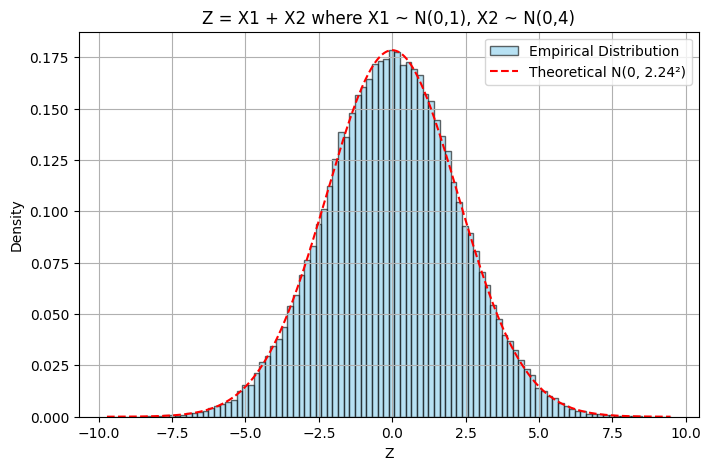
\includegraphics[width=0.8\linewidth]{normal_0_4.png}

\section*{Observations}
\begin{itemize}
  \item The sum of two uniform distributions results in a triangular or trapezoidal-like distribution.
  \item The sum of two normal distributions results in another normal distribution with mean and variance equal to the sum of the respective means and variances.
  \item In the case of mixed parameter ranges (e.g., \( U(0,1) + U(0,2) \)), the shape of \( Z \)'s distribution becomes more spread and asymmetric.
\end{itemize}

\section*{Conclusion}
This experiment demonstrates how the addition of independent random variables affects the resulting distribution. It provides a hands-on understanding of convolution of probability distributions and the central limit behavior.

\end{document}
